\scanpage{36}
On aura donc additivement
\[
(\unsure{\alpha})\qquad H^*(Y)=\coprod_{\substack{i+j\leq n-1\\i,j\geq0}}L_X^jP^i(X)\oplus E^{n-1}.
\]
L'opération
\[\varphi_*:H^*(Y)\longrightarrow H^*(X)\]
s'identifie donc à $L_X$ sur le morceau
\[\coprod_{\substack{i+j\leq n-1\\i,j\geq0}}L_X^j\unsure{P^j|P^i}(X)\]
du premier morceau de $(\unsure{\alpha})$, (et est \deleted{\unsure{un isom}} donc injectif sur ce morceau) et il est \uline{nul} sur le morceau
\[
\deleted{\coprod_{\unsure{0\leq i\leq n-1}}L_X^{\unsure{n-i}}P^{\unsure{i}}(X)\unsure{\oplus}}E^{n-1},
\]
\deleted{qui correspond \unsure{par l'isom can.} à $\displaystyle\sum_{\unsure{n-1\leq i\leq2(n-1)}}P^i(Y)$}. Ainsi on trouve le

\uline{Corollaire}
\[
\begin{aligned}
\operatorname{Ker}\varphi_*&=\deleted{\coprod_{\unsure{n-1\leq j\leq2n-1}}P^{\unsure{j}}(Y)\unsure{\simeq\operatorname{Ker}}}E^{n-1}(Y)\\
\operatorname{Im}\varphi_*&=\operatorname{Im}L_X=\bigcap_{0\leq i\leq n}\operatorname{Ker}p_i^X.
\end{aligned}
\]
(la dernière formule, car $H^*(Y)=\operatorname{Im}\varphi^*+E^{n-1}$ et $\varphi_*$ s'annule sur $E^{n-1}$, donc $\operatorname{Im}\varphi_*=\operatorname{Im}\varphi_*\varphi^*\unsure{\deleted{=I}}$, or $\varphi_*\varphi^*=L_X$).
\[
\left\{\begin{aligned}
p_i^X\varphi_*&=0 &&\text{si }0\leq i\leq n\\
p_{\unsure{j}}^X\varphi_*&=\varphi_*p_{\unsure{j}-2}^Y &&\text{si }\unsure{n+1}\leq i\leq2n.
\end{aligned}\right.
\]
On a
\[
\left\{\begin{aligned}
\varphi^*L_X&=L_Y\varphi^*\\
L_X\varphi_*&=\varphi_*L_Y
\end{aligned}\right.
\qquad
\varphi_*\varphi^*=L_X,\quad\varphi^*\varphi_*=L_Y
\]
formule de projection

\margin{\figure{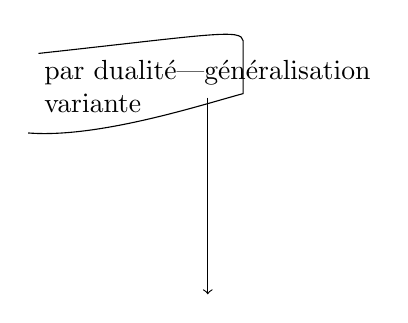
\begin{tikzpicture}[x=1cm,y=1cm]
\node[align=left,anchor=north west] (a) at (0,0) {\deleted{\unsure{par dualité|généralisation}}\\\unsure{variante}};
\draw (-.08,-1.05)..controls(.8,-1.12)and(2.1,-.7)..(2.65,-.55)--(2.65,.12)..controls(2.63,.28)and(2.25,.2)..(.05,-.04);
\draw[->] (2.2,-.6)--(2.2,-3.1);
\end{tikzpicture}}}
\deleted{Pour la dernière formule, \unsure{on note que les deux mbs} sont nuls sur $E^{n-1}$, donc il suffit de vérifier
\[
(L_X\varphi_*)\varphi^*=(\varphi_*L_Y)\varphi^*\quad\text{i.e.}\quad
L_X(\varphi_*\varphi^*)=\varphi_*(L_Y\varphi^*)=\inserted{\varphi_*\varphi^*L_X}
\]
car les deux mbs sont $L_X^2$.}
\mspage{35}
